\documentclass{beamer}

\usepackage[utf8]{inputenc}
\usepackage[T1]{fontenc}
\usepackage{listings}
\usepackage{xcolor}
\usepackage{graphicx}

%New colors defined below
\definecolor{codegreen}{rgb}{0,0.6,0}
\definecolor{codegray}{rgb}{0.5,0.5,0.5}
\definecolor{codepurple}{rgb}{0.58,0,0.82}
\definecolor{backcolour}{rgb}{0.95,0.95,0.92}

%Code listing style named "mystyle"
\lstdefinestyle{mystyle}{
  backgroundcolor=\color{backcolour},   commentstyle=\color{codegreen},
  keywordstyle=\color{magenta},
  numberstyle=\tiny\color{codegray},
  stringstyle=\color{codepurple},
  basicstyle=\ttfamily\footnotesize,
  breakatwhitespace=false,         
  breaklines=true,                 
  captionpos=b,                    
  keepspaces=true,                 
  numbers=left,                    
  numbersep=5pt,                  
  showspaces=false,                
  showstringspaces=false,
  showtabs=false,                  
  tabsize=2
}

\lstset{style=mystyle}

\usetheme{Madrid}
\usecolortheme{default}

\AtBeginSection[]{
  \begin{frame}
  \vfill
  \centering
  \begin{beamercolorbox}[sep=8pt,center,shadow=true,rounded=true]{title}
    \usebeamerfont{title}\insertsectionhead\par%
  \end{beamercolorbox}
  \vfill
  \end{frame}
}

\title{Vertx}
\author{Rafael Merino García}
\institute{@imrafaelmerino}
\date{2021}


\begin{document}

\frame{\titlepage}

\begin{frame}
\frametitle{Table of Contents}
\tableofcontents
\end{frame}

\section{Goals}

\begin{frame}
\frametitle{Goals (I)}
\begin{itemize}
    \item<1-> How to use  \textbf{Vertx} following the \textbf{Erlang} philosophy (\textbf{message passing})
    \begin{itemize}
        \item<2-> Why? \textbf{Low coupling} and  
        \item<3-> How do you get programs to run faster  \textbf{without changing a single line?}
            \begin{itemize}
               \item<4-> Increasing CPU frequency?      
               \item<5-> Increasing number of cores?
               \item<6-> Increasing number of machines?
            \end{itemize}    
     \end{itemize}    
    \item<7-> Understand better functional and reactive programming
    \begin{itemize}
        \item<8-> FP shines dealing with \textbf{effects}       
        \item<9-> Is your app really reactive? 
            \begin{itemize}
                 \item<10-> What's your first integration test?      
                 \item<11-> \textbf{Failures are just data}
           \end{itemize}   
    \end{itemize}    
\end{itemize}    
\end{frame} 


\begin{frame}
\frametitle{Goals (II)}    
    \begin{itemize}
    \item<1->  Develop complex services in Vertx \textbf{and not die trying} (async programming is still hard nowdays)
    \item<2->  A, B and C are http requests or database calls executed \textbf{in parallel} 
   \begin{figure}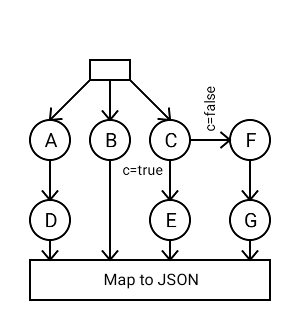
\includegraphics[scale=0.4]{images/flow-1.png}\end{figure}
     \item<3->  I didn't mention, but I was thinking of \textbf{just one line of code}
     \end{itemize}      
\end{frame} 


\begin{frame}
\frametitle{Goals (III)}    
 \begin{itemize}
    \item<1-> and if you retry some ops under certains errors (connection timeouts, network partitions etc) or want to add some action without waiting for the response, like sending an email (H)
    \begin{figure}
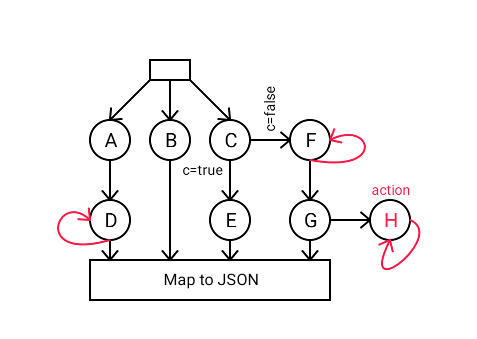
\includegraphics[scale=0.4]{images/flow-2.png}
\end{figure}
     \item<2->  I'm still thinking of just one line of code
     \end{itemize}    
\end{frame} 


\section{History}

\begin{frame}
\frametitle{Actor Model (1973)}
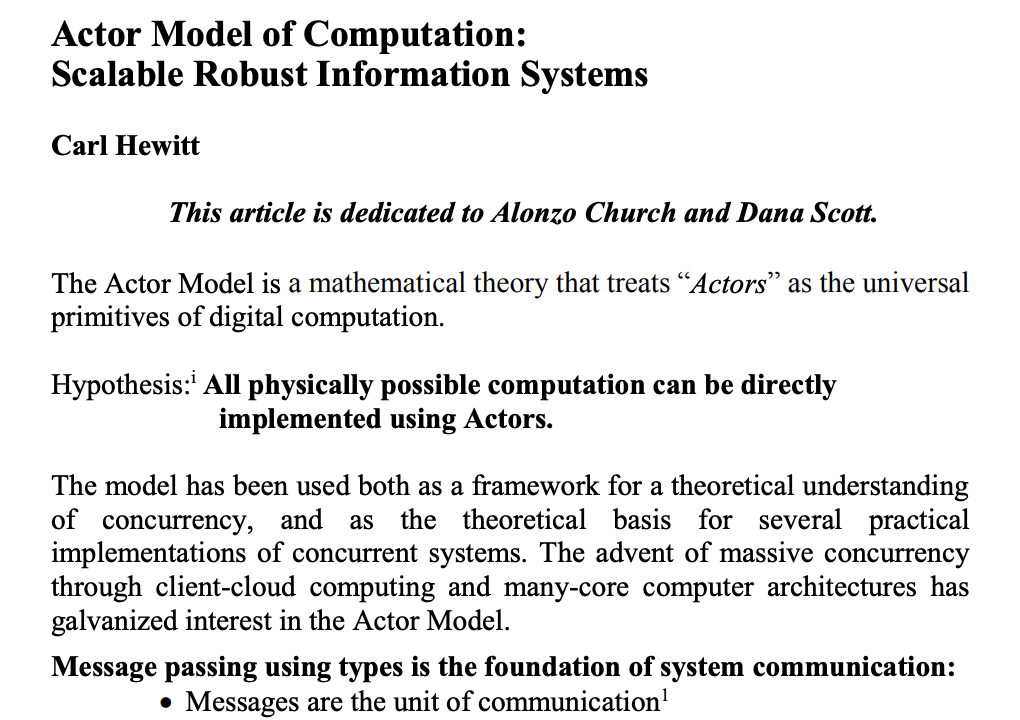
\includegraphics[scale=0.5]{images/actor_model_paper.png}
\end{frame}

\begin{frame}
\frametitle{SmallTalk (1970-1980)}
   \begin{itemize}
    \item<1->  \textbf{Alan Kay}, one of its creator, \textbf{coined the term Object Oriented Programming }but...   
    \item<2->  “I’m sorry that I long ago coined the term “objects” for this topic because it gets many people to focus on the lesser idea. \textbf{The big idea is messaging}.”
    \item<3-> "I made up the term ‘object-oriented’, and I can tell you \textbf{I didn’t have C++ in mind}.”
     \item<4-> Download Pharo and be blown away!
   \end{itemize}      
\end{frame}

\begin{frame}
\frametitle{Erlang (1986)}
   \begin{itemize}
    \item<1->  Open Source in 1998      
    \item<2->  Functional programming language created \textbf{to build fault-tolerant and scalable distributed systems in Ericsson}
    \item<3->  Isolated processes that \textbf{interact sending messages} (10 servers handling 1 req instead of 1 server handling 10 req)
    \item<4->  Keep calm and \textbf{let it crash} (avoid defensive programming and don't make things worse)
    \item<5-> WhatsApp  and WeChat are implemented in Erlang!
  \end{itemize}      
\begin{figure}
\end{figure}
\end{frame} 

\begin{frame}
\frametitle{Influential people}
\begin{figure}
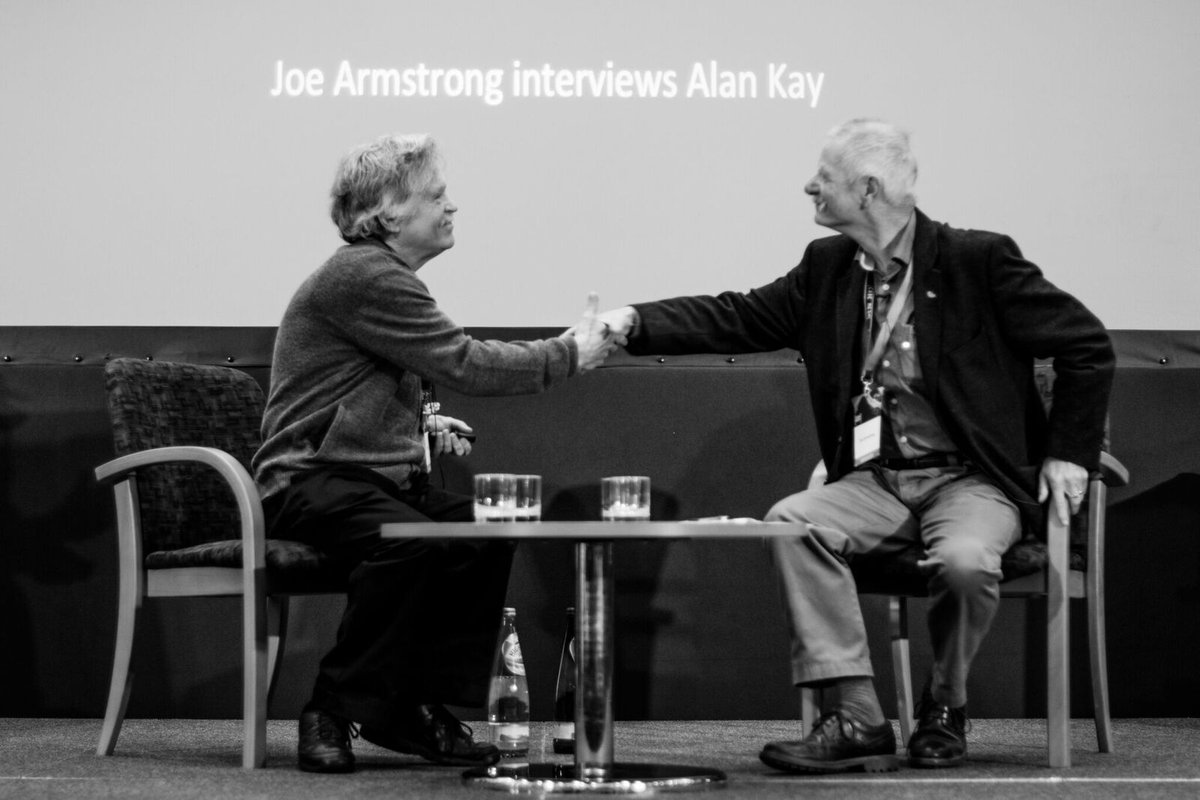
\includegraphics[scale=0.25]{images/joe_and_alan.jpg}
\end{figure}
\end{frame} 

\section{Vertx}

\begin{frame}
\frametitle{Recomendations (my own)}
\begin{itemize}
\item<1-> Understand what message passing means. \textbf{Adoption of a new paradigm is a complex and slow process that has to hurt}.
\item<2-> EOOP just doesn't fit (\textbf{don't use Spring or try to avoid it})
\item <3->Dependency injection == Coupling
\item<4-> \textbf{Have a plan to handle complexity}.
\end{itemize}
\end{frame} 


\begin{frame}
\frametitle{Verticles}
\begin{itemize}
 \item<1-> \textbf{Everything} is a Verticle (minimum execution unit)
 \item<2-> computation | storage | communication
 \item<3-> Can create and kill other verticles
 \item<4-> Verticles are strongly \textbf{isolated} (share no resources)
 \item<5-> Verticles creation and destruction is a lightweight operation
 \item<6-> Verticles have \textbf{unique} addresses
 \item<7-> If you know the address  of a verticle you can send it a message
 \item<8-> Message passing is \textbf{the only way} for verticles to interact
 \item<9-> \textbf{The more verticles the better}
\end{itemize}
\end{frame}


\begin{frame}
\frametitle{Message passing}
\begin{itemize}
\item<1-> Message passing is assumed to be \textbf{atomic} which means that a message is either delivered in its entirety or not at all
\item<2-> Message passing between a pair of verticles is assumed to be ordered: \textbf{the messages will be received in the same order they were sent}
\item<3-> Messages \textbf{should not contain references to data structures contained within verticles}—they should only contain constants and/or address
\item<4->\textbf{send and pray} semantics. We send the message and pray that it arrives
\end{itemize}
\end{frame}

\begin{frame}
\frametitle{Vertx model (I)}
\begin{figure}
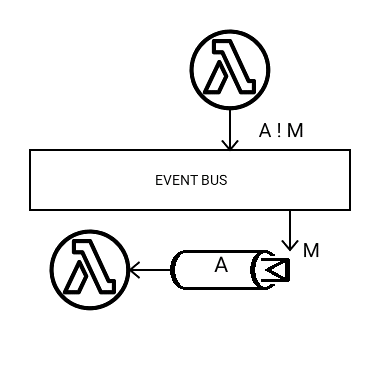
\includegraphics[scale=0.3]{images/vertx-model-1.png}
\begin{itemize}
\item<1-> The event bus  is the nervous system of Vertx
\item<2-> Distributed event bus: verticles \textbf{from different machines} can communicate with each other sending messages. Scale-out
\item<3-> It provides an API to:
\begin{itemize}
        \item<4-> deploy verticles listening on addresses
        \item<5-> \textbf{send and publish} messages to addresses: point-to-point and pub/sub 
\end{itemize}        
\item<6->  \textbf{Verticles process ONE message at a time}. Syncronization is implemented this way
\end{itemize}
\end{figure}
\end{frame}

\begin{frame}
\frametitle{Vertx model (II)}
\begin{figure}
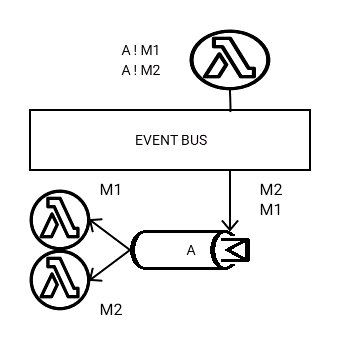
\includegraphics[scale=0.3]{images/vertx-model-2.png}
\begin{itemize}
\item<1-> Scale-up: deploying multiple instances of a verticle listening on the same address
\item<2-> Instance that receives the message is chosen using a non-strict round-robin algorithm 
\end{itemize}
\end{figure}
\end{frame}

\begin{frame}
\frametitle{Vertx model (III)}
Imagine that a verticle \textbf{sends a message} to other verticle and has to\textbf{ process the response}
\begin{itemize}
\item<1-> Programmatically, it's just a handler
\item<2-> but in practice it's just another verticle listening on a random address
\end{itemize}
\begin{figure}
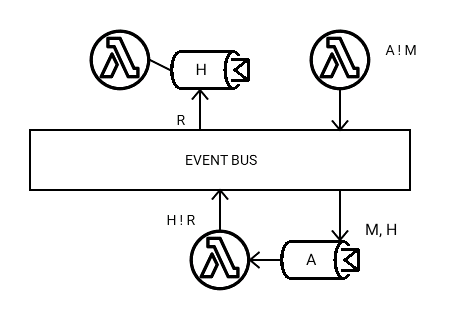
\includegraphics[scale=0.3]{images/vertx-model-3.png}
\end{figure}
\end{frame}

\begin{frame}
\frametitle{Verticles life cycle}
\begin{itemize}
\item<1-> Verticles that are created during app boostrap and never dye
\item<2-> Verticles that are associated to the life cycle of an entity (user login and logout)
\item<3-> Verticles that  are created to do computation and die after that. Why do we need an address then?
\end{itemize}
\end{frame}

\begin{frame}
\frametitle{Messages}
\begin{itemize}
\item<1-> String, null, bytes, Numbers, Boolean and Json (from Jackson)
\item<2-> All supported messages have a MessageCodec associated
\item<3-> You can send your own messages if you create and register their codecs
\item<4-> The vertx Json is mutable. ¿Why is this a problem?
\begin{itemize}
\item<5-> Verticles have to be isolated
\newline
\begin{figure}
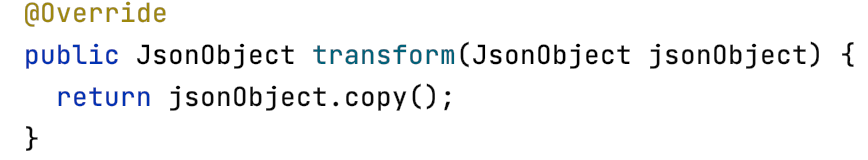
\includegraphics[scale=0.5]{images/vertx-json-codec.png}
\end{figure}
\end{itemize}
\item<6->  imrafaelmerino/json-values is a better alternative: it's persistent and provides a better api
\newline
\begin{figure}
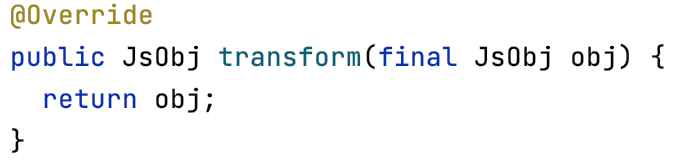
\includegraphics[scale=0.5]{images/jsvalues-codec.png}
\end{figure}
\end{itemize}
\end{frame}

\begin{frame}
\frametitle{Threading model}
\begin{itemize}
\item<1->Two type of threads: \textbf{event loops and workers}
\item<2-> When deploying a verticle you have to specify if it will be executed by      
 a worker or an event loop
\item<3-> computationally intensive or blocking tasks $\Rightarrow$ worker
 \item<4-> never block an event loop
 \item<5-> Size of pools by default
 \begin{itemize}
          \item<6->event loops: 2 x processors
          \item<7->workers: 20
          \item<8->What's the right size?
 \end{itemize}     
 \item<9-> What about green threads and project Loom?    
\end{itemize}
\end{frame}


\section{vertx-effect: where Vertx meet FP }
\begin{frame}
\frametitle{Vertx future}
 \begin{itemize}
          \item<1->Vertx 4 use futures to represent asynchronous results, but
          \item<2-> Vertx future API \textbf{is not rich enough} to develop complex verticles:
\item<3->\textbf{Only three methods to coordinate}: join, all and any
\item<4-> Since \textbf{it's not lazy}, key reactive operations like \textit{retry}, \textit{recoverWith} and \textit{fallbackTo} are missing                       

 \end{itemize}   
\end{frame}

\begin{frame}[fragile] 
\frametitle{Val and $\lambda$ }
\begin{lstlisting}[language=Java,numbers=none,mathescape=true]
import java.util.function.Supplier;
import java.util.function.Function;
import io.vertx.core.Future;

public interface Val<O> extends Supplier<Future<O>> {...}

public interface $\lambda$<I,O> extends Function<I, Val<O>> {...}

\end{lstlisting}

\clearpage

\begin{itemize}
 \item<1->  Val is \textbf{lazy}. It \textbf{describes} an asyncronous effect
 \item<2-> The types \textbf{I} and \textbf{O} represent messages sent to the Event Bus 
 \item<3-> If they are not supported by Vertx
       \begin{itemize}
        \item<4-> Implement and register a \textbf{MessageCodec} for them
      \end{itemize}
 \end{itemize}

\end{frame}


\section{Practice makes perfect}

\begin{frame}
\frametitle{Hands-on}
\begin{itemize}
\item<1->  Playing around with values
\item<2->  Expressions
\item<3->  Lambdas
\item<4->  Deploying verticles and modules
\item<5->  Reactive http client
\item<6->  Wrapping existing libraries with lambdas: vertx-mongodb-effect
\item<7->  Implementing complex flows
\end{itemize}

\end{frame}

%Bibliographic references
\begin{thebibliography}{9}
\bibitem{latexcompanion} 
Michel Goossens, Frank Mittelbach, and Alexander Samarin. 
\textit{The \LaTeX\ Companion}. 
Addison-Wesley, Reading, Massachusetts, 1993.

\bibitem{einstein} 
Albert Einstein. 
\textit{Zur Elektrodynamik bewegter K{\"o}rper}. (German) [\textit{On the electrodynamics of moving bodies}]. 
Annalen der Physik, 322(10):891–921, 1905.

\bibitem{knuthwebsite} 
Knuth: Computers and Typesetting,
\\\texttt{http://www-cs-faculty.stanford.edu/\~{}uno/abcde.html}
\end{thebibliography}




\end{document}





